\chapter{Computational Complexity} \label{chap:computational-complexity}

The goal of optimization is to find the best solution to a problem.  However, in many practical cases, the quality of the solution may be a less important factor than the total resources that must be expended in finding the solution.   There is a large field of research which focuses on this issue of \textit{computational complexity}: how long will it take to solver a problem, or can the problem be solved at all?

One popular categorisation of optimisation/decision problems is linked to the concept of a Turing Machine (TM), depicted in Fig.~\ref{fig:TM}. This is a  construct introduced in a landmark paper by Alan Turing in the 1930s \cite{turing1937computable}, in which he provided a proof that certain decision problems are \textit{undecidable}.  A TM is a device with a read/write head which, at any point in time, points to a single location on a tape of symbols.  All symbols on the tape come from a finite alphabet $\Sigma_{\text{tape}}$ (in the figure, the alphabet contains three symbols, $\Sigma_{\text{tape}} = \{0, 1, b\}$, where $b$ is used to denote a blank space).  In addition to being able to read and write from the tape, the machine itself maintains a state, which consists of a symbol $s_i$ from a second finite alphabet, $\Sigma_{\text{machine}} = \{s_1, \dots, s_m\}$. Finally, it has access to a set of instructions which take the form: \textit{if the tape symbol is $t_i$ and the state symbol is $s_i$, then write symbol $t_j$ to the current position, change state to $s_j$ and move one step in direction $D$}.  Here the direction can be L (left) or R (right).  An instruction can be therefore written as a $5$-tuple $(t_i, s_i, t_j, s_j, D)$.  The machine continues to run until it reaches a predefined \textit{accepting state}. There is a full worked example of writing a program that leads to a Turing machine copying an input sequence in \cite{turingMachines}.



\begin{figure}
\centering
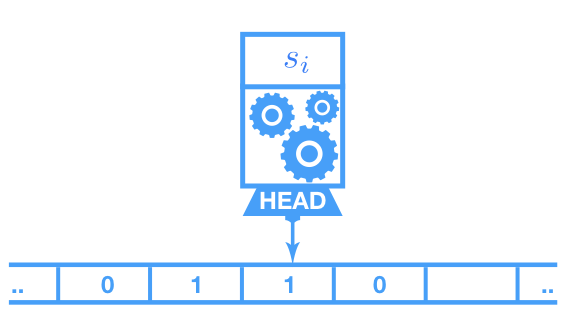
\includegraphics[width=0.5\textwidth]{figs/turing-machine-fig-001.png}
\caption{The Turing machine: a simple device with a read/write head which points to a single cell location on a tape of symbols.  The machine maintains a single state (currently $s_i$). \label{fig:TM}}	
\end{figure}

For the purposes of analysing the complexity of a program, we can define two distinct types of Turing machine. The first is the \textit{deterministic} Turing machine (DTM).  For any given machine state and tape symbol pairing, the instructions for the DTM can prescribe at most one action. The second type of machine is the \textit{non-deterministic} Turing machine (NTM), which allows instructions to specify multiple actions as outcomes for a given input configuration.  Both machines have the same \say{power}, in the sense that they can both solve the same types of problems.  However, the speed at which they can solve them can differ dramatically.  At each instruction with multiple outcomes, the NTM can branch (we can think of the machine as cloning itself and sending one clone along each output action), enabling it to explore an exponentially large space of execution paths.  By contrast, the DTM may only proceed along a single execution path at a time.  These concepts are useful because they provide a way to describe which problems are \say{exponentially expensive}.

Specifically, we define the class of decision problems \textit{P}, as those that can be solved by a DTM in polynomial time (by which we mean that the time is a polynomial function of the input).  We further define the class \textit{NP}, as those that can be solved by an NTM in polynomial time (the \say{N} here stands for non-deterministic). It is also popular to use the equivalent definition of NP as the set of problems that can be \textit{verified} in polynomial time by a DTM (intuitively, we can imagine following just the branch taken by the NTM clone that eventually reaches the accepting state with a single DTM).  The question of whether these two problem classes are equivalent is considered one of the classic (unsolved) problems of computer science \cite{pvnp}.

There are two further categories which are often used to describe problem complexities. A problem $t$ is said to be \textit{NP-hard} if it satisfies the property that any problem in NP can be reduced to problem $t$ in \textit{polynomial time} by a DTN.  A problem is said to be \textit{NP-complete} if, in addition to being NP-hard, it also lies in NP.  